% Created 2023-03-05 Sun 17:15
% Intended LaTeX compiler: xelatex
\documentclass[manuscript,screen,review]{acmart}


\bibliographystyle{ACM-Reference-Format}
\author{30093813}
\date{\today}
\title{NLP Milestone}
\hypersetup{
 pdfauthor={30093813},
 pdftitle={NLP Milestone},
 pdfkeywords={},
 pdfsubject={},
 pdfcreator={Emacs 28.2 (Org mode 9.5.5)},
 pdflang={English}}
\usepackage{natbib}
\begin{document}

\maketitle
\section*{Introduction}
\label{sec:orga8d7a2c}
This project will attempt to address the problems resulting from the
necessity for manual linking in educational material. In particular,
educational material often requires large amounts of repetitive
linking to related explanatory material as it uses domain-specific
terminology. This project will explore the NLP techniques that can be
used to enable the automatic identification of the spans of a document
which should be linked, and the pairing of such spans with their
appropriate links.

\section*{Solution}
\label{sec:orgcb75316}
The work on the project so far has consisted mainly of data
preparation, with some minor initial exploration done into model
training with SpaCy.

The dataset chosen was the \texttt{scikit-learn} documentation (GitHub source:
\url{https://github.com/scikit-learn/scikit-learn/tree/main/doc}, commit
\texttt{449940985c903f77678c0627cbc7a6267c3a54f9}). To extract the link data
from the documents, I wrote a tool which uses Pandoc to assign UUIDs
to each link in each document, wrap the link content with a special
marker for later extraction, store the UUID-to-link mapping in a JSON
file, and convert the HTML to plain text. Pandoc was chosen to make it
easier to use the tool on different datasets with different
documentation formats.

After that, Python is used for further processing of the links. The
dataset consists of 996 documents with a total length of 1100122 words
(according to the \texttt{wc} command line utility). Unprocessed, the dataset
consists of a total of 17982 unique links. Multiple processing steps
were used to account for different link forms: the links were
lowercased, "http" forms of existing "https" links were converted to
"https", Python's \texttt{urllib} was used for normalization, and relative
links were normalized. Following this processing, the dataset
consisted of 17164 unique links.

The majority of links have very few occurences; \ref{fig:orgb64256e}
illustrates the exponentially decreasing relationship between the
minimum occurence count and the number of classes meeting that
minimum. More than half the links in the dataset have only one
example, and only 474 out of the \textasciitilde 17000 links have more
than 10 examples.

\begin{figure}[htbp]
\centering
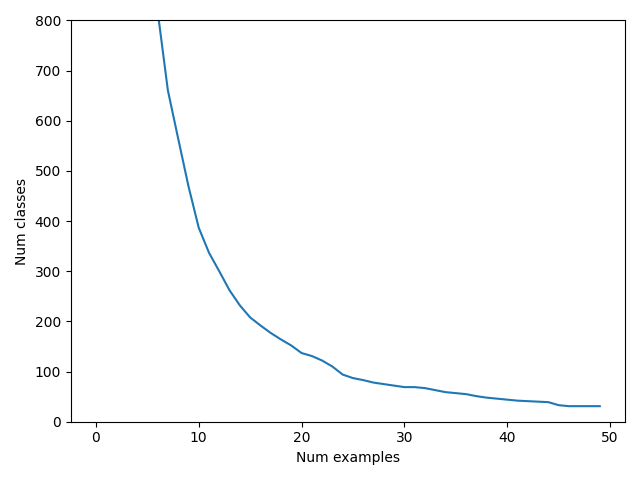
\includegraphics[width=.9\linewidth]{images/numclasses.png}
\caption{\label{fig:orgb64256e}Distribution of minimum example count}
\end{figure}

To help reduce the number of classes, we can focus on the links with
many examples; fortunately this is suitable for the application,
because links with many examples are more likely to be used again.

There is also the issue of splitting the data into training and
testing data. For this task I wrote a script which provides a roughly
balanced split of the documents in the dataset, in terms of their
example counts for each class. The script accepts a test size and a
minimum example threshold, and performs a search for a balanced
split. The split class statistics are summarized in \ref{tab:orgf98d89e}. A
minimum example threshold will be chosen based on model results, but
these initial findings indicate that 15 may be a good threshold.

\begin{table}[htbp]
\caption{\label{tab:orgf98d89e}Counts of classes in training and test sets for different thresholds}
\centering
\begin{tabular}{rrrr}
Minimum examples & \# Training set classes & \# Testing set classes & \# Classes with no test examples\\
\hline
5 & 1152 & 1029 & 123\\
10 & 474 & 466 & 8\\
15 & 274 & 273 & 1\\
20 & 181 & 180 & 1\\
25 & 123 & 122 & 1\\
30 & 104 & 104 & 0\\
\end{tabular}
\end{table}

After the data is split into training and testing sets, another script
extracts the link locations from the plain text files and creates
SpaCy \texttt{Doc}'s annotated with the link locations and their link
labels. These \texttt{Doc}'s are stored in SpaCy's binary data format so that a
SpaCy pipeline can be trained on the data.

Thus far, a single pipeline has been trained on the minimum 15
threshold dataset with a \texttt{tok2vec} component and a \texttt{spancat} (span
categorizer) component predicting links, with the best model reaching
and F-score of \textasciitilde 0.8. This score may not reflect the
actual utility of the model, as the extraneous links described in
\hyperref[sec:orgd811032]{Challenges} may be boosting the score. It was not possible to train the
pipeline with the default configuration on unpaid Google Colab due to
limited memory, but I was able to train it on my laptop on CPU. This
pipeline was an initial experiment to confirm the data was in an
appropriate format for training. Over the following month I will be
further researching the training process in SpaCy and evaluating
different models.

\section*{Challenges}
\label{sec:orgd811032}

The documentation for \texttt{scikit-learn} is in RST format, and it has a
build tool in place which allows special link types. This makes it so
that the full hyperlinks cannot be parsed directly from the RST
source, so instead I have taken the built HTML source and parsed the
links from there. This has the downside that extraneous hyperlinks,
such as those in the navigation bar, may need to be excluded as a
special case. This special case will be explored based on the model
results. If these hyperlinks need to be removed, it will be possible
by limiting the parsed HTML to only those within the tag representing
the main content of the webpage.

Another unanticipated challenge came with splitting the documents into
train and test data such that the classes were balanced. The
combination of a large number of classes, a large imbalance in the
number of examples for the different classes, and an unequal
representation of the classes across documents made it challenging to
find a balance, and I couldn't find an existing tool for the task. I
was able to write a search for this, but it doesn't always find a
perfect balance. If the split ends up being unsuitable, the search can
be applied to split by paragraph instead of document, or possibly by
sentence, depending on the amount of context required by the model.
\end{document}